\documentclass[preview,border=5pt]{standalone}
\usepackage{teaching}
\begin{document}

\centering

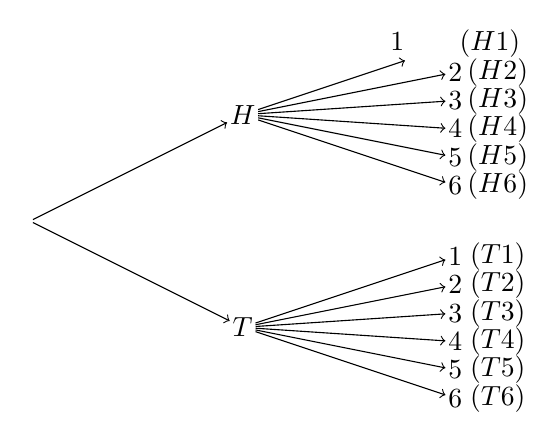
\begin{tikzpicture}[yscale=1,xscale=1,scale=1.8,inner sep=0.3mm, label distance=1.5mm]

\node(o) at (-1.5,0) {};
\node(h) at (0,0.75) {$H$};
\node(t) at (0,-0.75) {$T$};
\draw[->] (o) -- (h);
\draw[->] (o) -- (t);

\node(a1) at (1.5,1.25) {$1\qquad(H1)$};
\node(a2) at (1.5,1.05) {$2$};
\node(a3) at (1.5,0.85) {$3$};
\node(a4) at (1.5,0.65) {$4$};
\node(a5) at (1.5,0.45) {$5$};
\node(a6) at (1.5,0.25) {$6$};

\node(b1) at (1.5,-1.25) {$6$};
\node(b2) at (1.5,-1.05) {$5$};
\node(b3) at (1.5,-0.85) {$4$};
\node(b4) at (1.5,-0.65) {$3$};
\node(b5) at (1.5,-0.45) {$2$};
\node(b6) at (1.5,-0.25) {$1$};

%\node(h1) at (1.8,1.25) {$(H1)$};
\node(h2) at (1.8,1.05) {$(H2)$};
\node(h3) at (1.8,0.85) {$(H3)$};
\node(h4) at (1.8,0.65) {$(H4)$};
\node(h5) at (1.8,0.45) {$(H5)$};
\node(h6) at (1.8,0.25) {$(H6)$};

\node(t1) at (1.8,-1.25) {$(T6)$};
\node(t2) at (1.8,-1.05) {$(T5)$};
\node(t3) at (1.8,-0.85) {$(T4)$};
\node(t4) at (1.8,-0.65) {$(T3)$};
\node(t5) at (1.8,-0.45) {$(T2)$};
\node(t6) at (1.8,-0.25) {$(T1)$};


\draw[->] (h) -- (a1);
\draw[->] (h) -- (a2);
\draw[->] (h) -- (a3);
\draw[->] (h) -- (a4);
\draw[->] (h) -- (a5);
\draw[->] (h) -- (a6);

\draw[->] (t) -- (b1);
\draw[->] (t) -- (b2);
\draw[->] (t) -- (b3);
\draw[->] (t) -- (b4);
\draw[->] (t) -- (b5);
\draw[->] (t) -- (b6);

\end{tikzpicture}

\end{document}